\section{问题分析与系统框架}
我国多能源系统同时受需求增长、数年建设时滞与小时供给波动影响。赛题的三个问题对应一条决策链：以历史现状建立统一初态，以多主体演化评价双碳路径，再以安全约束筛查投资和运行方案\cite{contest}。

本文将煤、油、气及电力服务需求与七类电源、两类储能和三类燃料供应资产统一到资源清算环境。政府通过碳价传递排放目标，消费载能群依据相对成本和上期缺供调整请求，投资主体依据分类运行反馈提出订单；订单经资本与建设约束进入队列，经过建设后形成供能能力。关键年快照进一步进入连续小时仿真，追踪能流、库存和债务的全过程。

\begin{figure}[H]\centering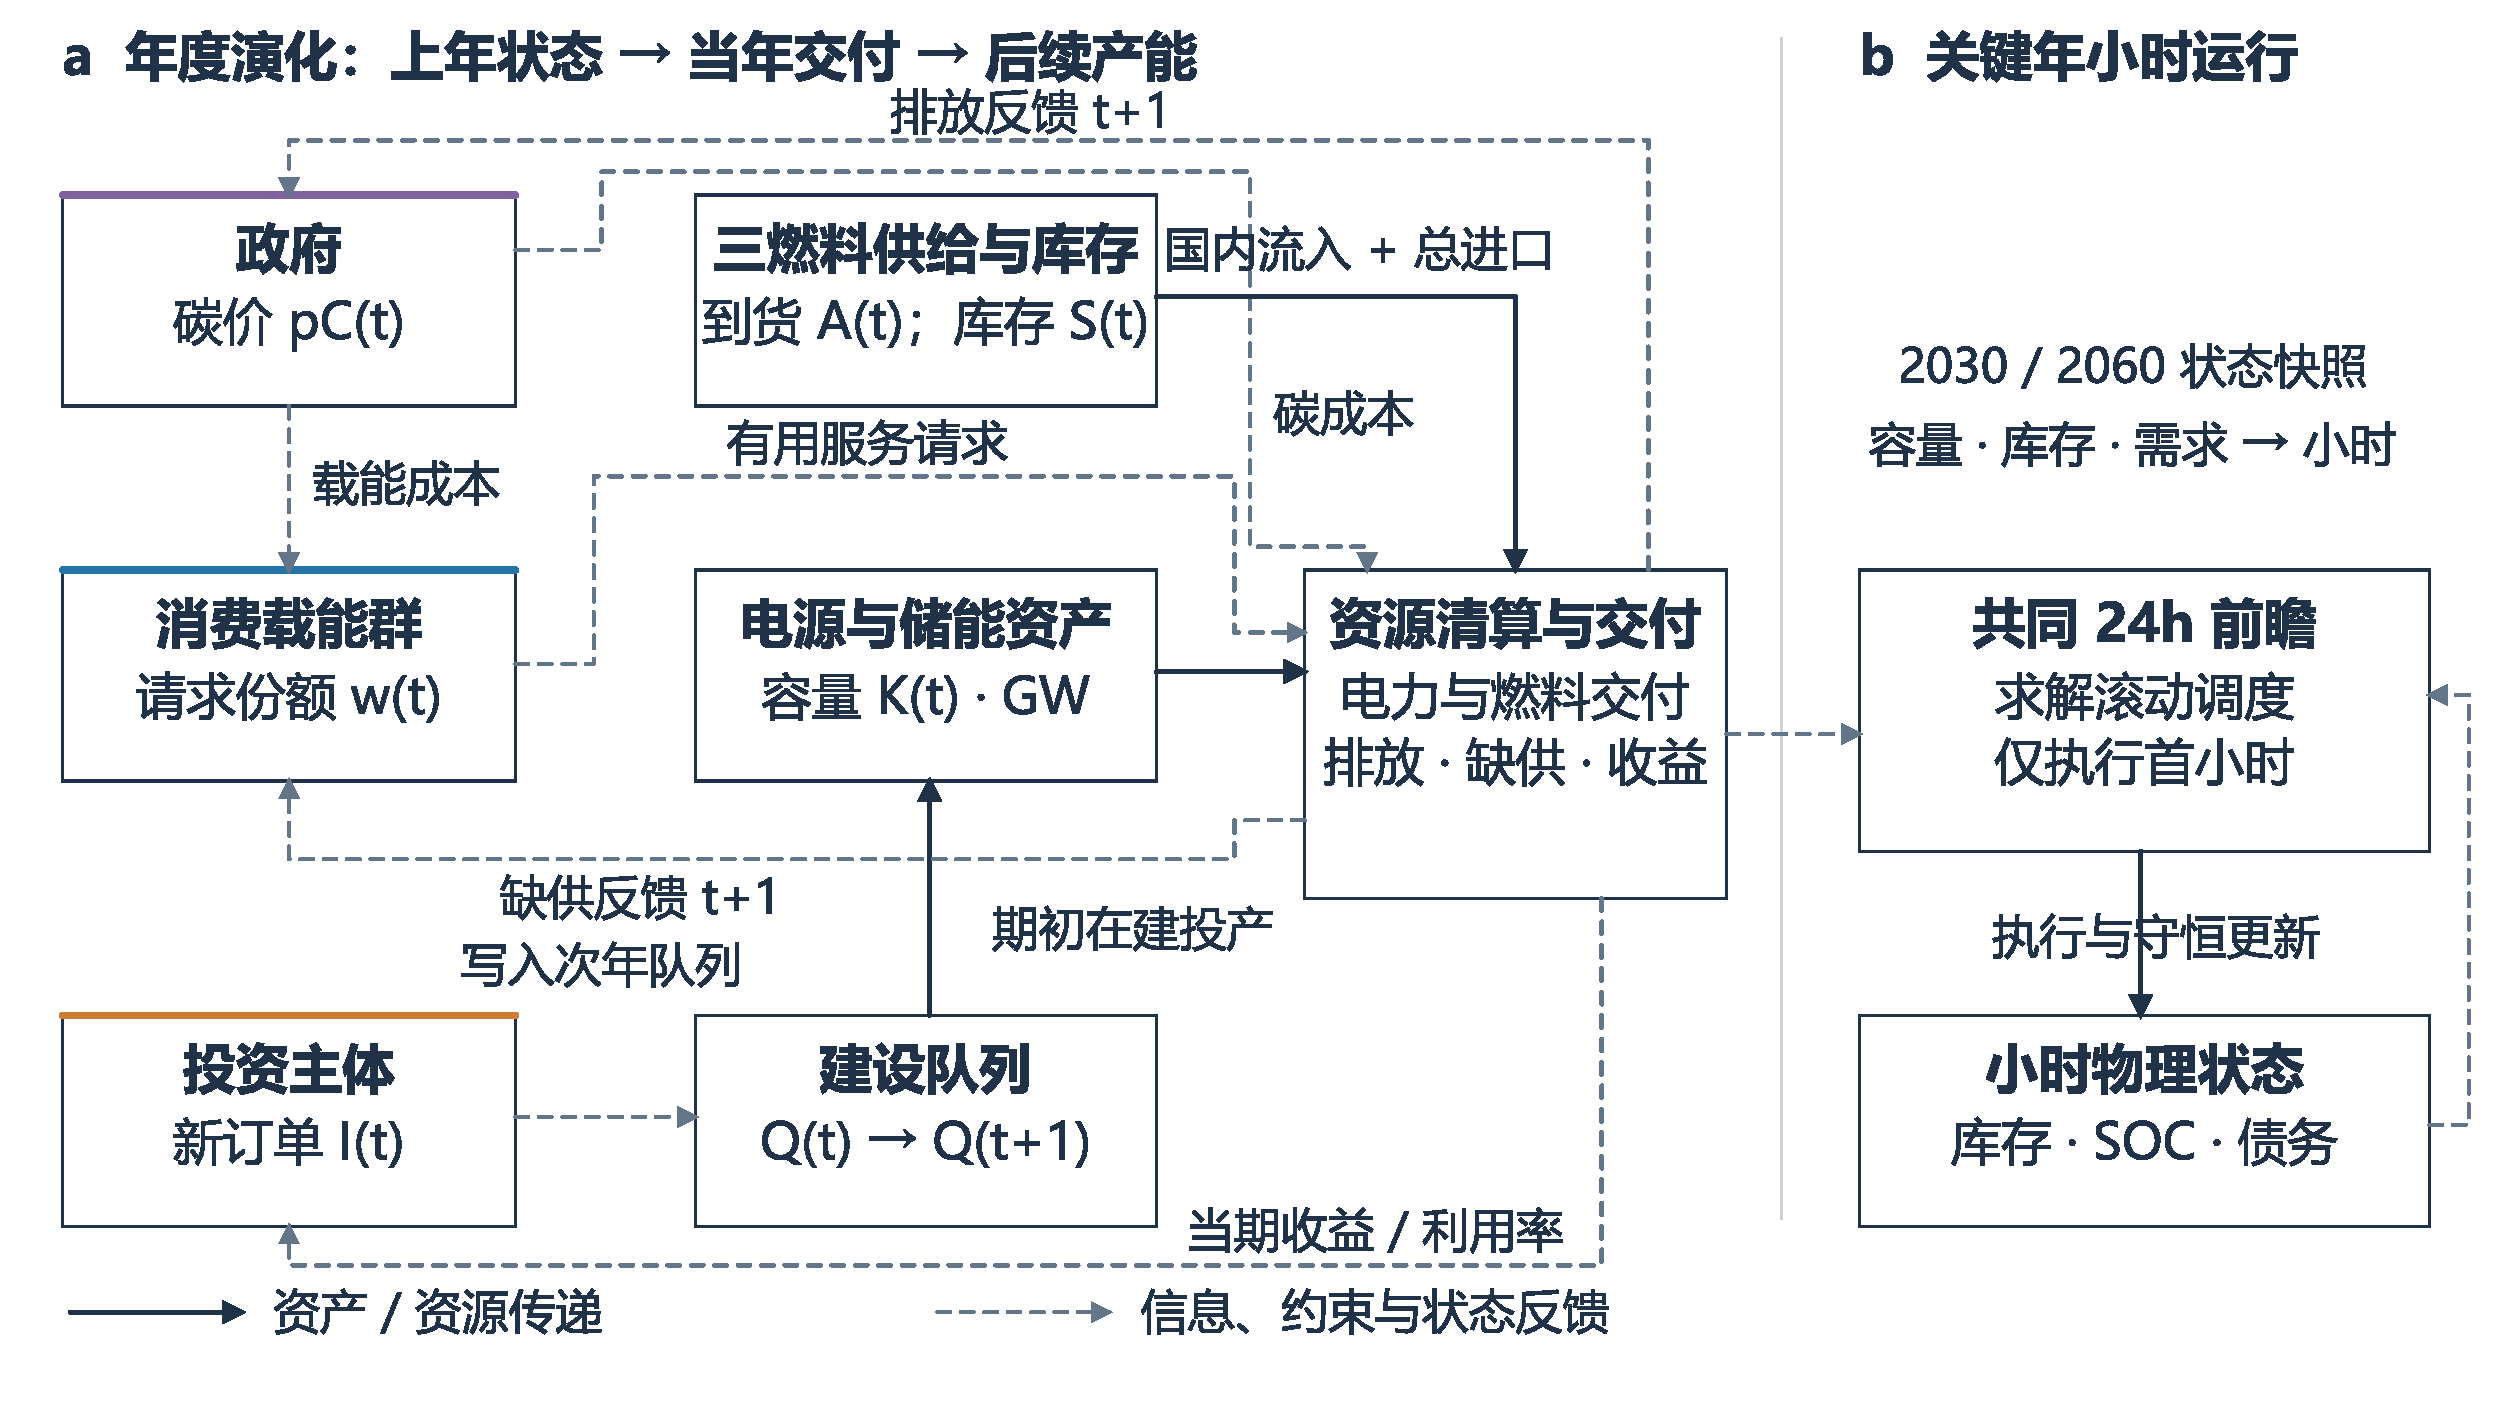
\includegraphics[width=\linewidth]{figures/fig01_system_architecture.pdf}\caption{主体决策—建设队列—资源清算—小时运行架构。实线表示物理状态或资源转移，虚线表示信息反馈；年度状态单向传入小时层。}\label{fig:fig01_system_architecture}\end{figure}


\textbf{长期转型路径能否成立，不仅取决于2060年的技术结构，还取决于此前每一年形成的供能能力及其安全约束。}因此，本文先由历史变化识别供给与结构矛盾，再用主体反事实解释长期结果，最后同时检验投资路径的逐年交付和冲击后的资源恢复。

\begin{table}[H]\centering\caption{三问的决策链与检验证据}
\begin{tabularx}{\linewidth}{p{.16\linewidth}XX}\toprule
任务 & 进入下一环节的结果 & 对应证据\\\midrule
现状评价 & 统一需求、装机、进口与库存初态 & 同版统计序列、分类口径与基年资源闭合\\
双碳推演 & 主体动作经建设队列形成关键年系统状态 & 共享历史组件、全因子机制对照与四情景指标\\
安全优化 & 投资路径筛查后，从相同初态比较运行规则与补库 & 固定方案扰动、原生反馈、强基线、能量守恒与多目标约束\\
\bottomrule\end{tabularx}\end{table}
